\chapter{Theory}

\section{Helical resonator models}
In order to create a helical resonator satisfying experimental conditions and limitations we inevitably come to a need for a theoretical model that would be able to predict essential characteristics of a resulting unit. The following sections aim to provide an overview and comparison of those.

\subsection{Macalpine \& Schildknecht}
\begin{figure}[h]
	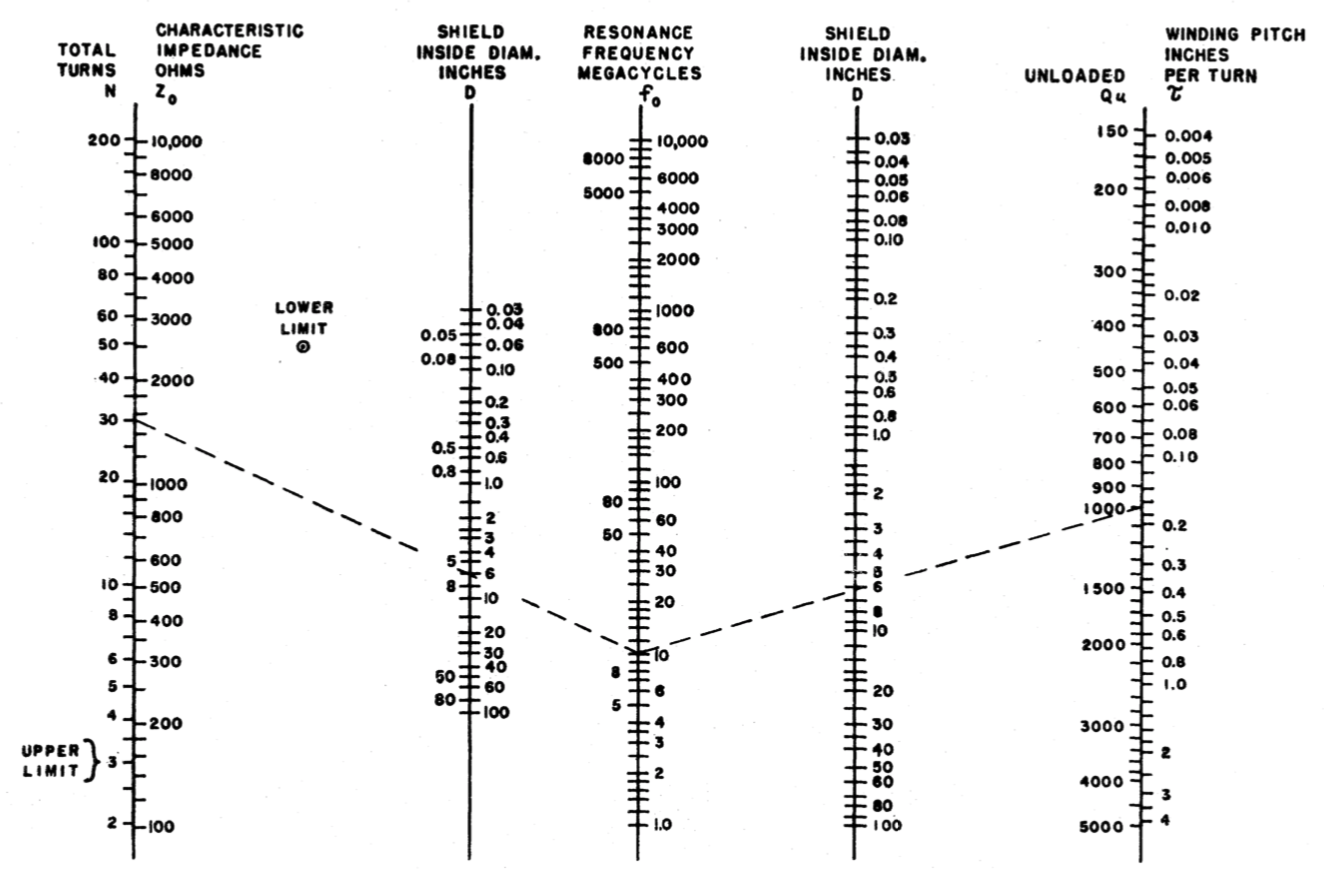
\includegraphics[width=\textwidth]{images/macalpine_chart}
	\caption{Design chart for quarter-wave helical resonators.}
	\label{fig:macalpine_chart}
\end{figure}

A well-known approach \cite{Macalpine2000} for describing helical resonators was introduced in the same year as Richard Feynman's idea \cite{Feynman1960} to use quantum systems for computations. It was motivated by the possibility to reduce volume compared to TEM-mode coaxial-line resonators. While skipping a detailed theoretical analysis it nevertheless provides a basis for constructing a resonator: such as regions of usefulness, design considerations and a set of parameters' dependencies maximizing $Q$.

While describing essential properties of an unloaded helical quarter-wave resonator this paper \cite{Macalpine2000} also predicts shift of resonant frequency if an external load is connected. In order to define new frequency one can make use of telegraph equations \cite{Rohde2009} by effectively treating the ion trap as a capacitor.

\subsection{Siverns et al.}
This model \cite{Siverns2012} takes one step further to development of an amplifier specifically for the needs of quantum computing. Authors propose to take a look at the joint resonator--ion trap system as a whole. It allows to calculate proper resonant frequency, accounting for resistive losses.


\section{Comparison}

Macalpine uses a generic model for coaxial / helical resonator, later improving it by using telegrapher's equations to estimate resonant frequency shift. Hensinger takes a less generic approach, taking some resonator-only parameters from Macalpine but investigating helical resonator + ion trap system